\section{Introduction}
\label{sec:introduction}

Online anonymity is typically synonymous with \emph{client anonymity}; VPNs
promise to disguise one's IP address, An equally pressing requirement can be
\emph{server anonymity} when the operator of a site is facing harassment or legal
repercussions.  Decoupling a server's content from the identity of its operator
can mitigate these issues.  Several systems implement various flavours of server
anonymity, including I2P, Freenet, and X, but in this work we focus on Tor's
onion services.

The Tor anonymity network is primarily known as a tool that enables client
anonymity, \ie, it allows users who download the project's Tor Browser to
browse the web anonymously~\cite{Dingledine2004a}.  In addition to client
anonymity, Tor provides server anonymity in the form of onion services (\aka
hidden services) which allow operators to expose a TCP service over the Tor
network while hiding its IP address.

Onion services have grown substantially over the last years, both in the number
of services and users.  As of May 2017, The Tor Project's statistics show that
more than 50,000 onion services are online each day, relaying more than 750 MBps
of network traffic.  Not all of these services host web sites---other use cases
such as meta data-free messaging~\cite{ricochet} and file
sharing~\cite{onionshare} have emerged as well.  Learning the number of onion
service users is more challenging.  In 2016, Facebook reported that more than
one million users logged into their onion service over a one month
period~\cite{facebook-users}.
RFC~\cite{rfc7686}

Past usability research focused on Tor Browser~\cite{Clark2007a,Norcie2014a}
and Tor's censorship circumvention~\cite{Fifield2015a}.  The usability of onion
services remains mostly unexplored.

The most salient aspect of onion services is their peculiar domain names.
Being derived from RSA public keys, they consist of random Base32 characters
such as the following three examples.

\begin{figure}[t]
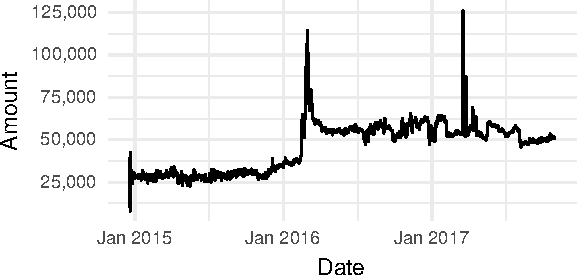
\includegraphics[width=\linewidth]{figures/os-growth.pdf}
\caption{The estimated median number of unique onion services per day since
2015.}
\label{fig:os-growth}
\end{figure}

{\footnotesize
\begin{verbatim}
6hylx55pr5dnod4t.onion
ke33kjltp3twmcwq.onion
4v4ndsnrjekbfhij.onion
\end{verbatim}
}

Onion domains are random, very difficult to remember, and cumbersome to work
with.  The next generation of onion services exacerbates this problem by
employing domains consisting of 54 (instead of sixteen) Base32-encoded
characters, giving them the following format:

{\footnotesize
\begin{verbatim}
lfels7g3rbceenuuqmpsz45z3lswakqf56n5i3bvqhc22d5rrszzwd.onion
llamanymityx4fi3l6x2gyzmtmgxjyqyorj9qsb5r543izcwymlead.onion
odmmeotgcfx65l5hn6ejkaruvai222vs7o7tmtllszqk5xbysolfdd.onion
\end{verbatim}
}

Properties that we take for granted in the non-onion web are not present in the
onion web.  The usability of onion services differs from ordinary websites in
the following aspects that we are trying to capture in our survey.  The first
issue is \emph{accessibility}.  Onion services are only accessible over Tor for
full client anonymity.\footnote{Services such as Tor2web allow normal web
clients to access onion services but that means that users give up client
anonymity~\cite{tor2web}.} The next issue is onion service \emph{discovery}.
It is difficult to learn about new onion sites.  There is no central directory,
and---unlike the web---onion sites do not link to each other
much~\cite{Griffith2017a}.  However, search engines such as ahmia.fi and
onion.link are a beginning.  Once users learn about new onion service, their
\emph{domain format} makes it difficult to memorize them.  Perhaps the most
salient idiosyncrasy of onion domains is that they are generated randomly.  As
a result, onion domains are difficult to memorize and recognize, forcing users
to handle them differently than normal websites.  Browsing onion sites may feel
clunky because of \emph{latency}---the number of hops in between Tor user and
onion service is causing tangible communication latency that many users may not
be willing to tolerate.

To date, only anecdotal evidence exists on how people interact with onion
services.  In this work we seek to fill this gap by administering a survey
designed to answer the following research questions: \emph{How do Tor users
interact with onion services?}  An answer to this research question allows us
to both create more usable anonymity systems and build these systems in a way
that semantic attacks such as phishing are exacerbated.\footnote{Downs \ea
distinguish between physical (\ie targeting physical infrastructure),
syntactic (\ie targeting software), and semantic (\ie targeting humans)
attacks~\cite[\S~1]{Downs2006a}.}  In particular, we seek to answer the
following three aspects:

%%%
In this paper, we answer our research question by conducting a survey.
We seek to inform X and Y to do Z better.
%%%

\begin{itemize}
    \item What is the expectation of privacy when people use Tor Browser in
        general and onion sites in particular?
    \item What is the security/usability trade-off of vanity onion domains?
    \item Do people handle onion domains differently than normal domains?
\end{itemize}

The rest of this paper is structured as follows.  We begin by discussing related
work in Section~\ref{sec:related-work}, followed by technical background in
Section~\ref{sec:background}.  Section~\ref{sec:survey-design} presents the
design of our survey and Section~\ref{sec:results} analyzes our results.  We
then discuss our results in Section~\ref{sec:discussion} and conclude in
Section~\ref{sec:conclusion}.
